
\documentclass{article}
\usepackage{spconf,amsmath,epsfig}
\usepackage{subfigure}

\let\OLDthebibliography\thebibliography
\renewcommand\thebibliography[1]{
  \OLDthebibliography{#1}
  \setlength{\parskip}{0pt}
  \setlength{\itemsep}{0pt plus 0.3ex}
}

\pagestyle{empty}


\begin{document}\sloppy

% Example definitions.
% --------------------
\def\x{{\mathbf x}}
\def\L{{\cal L}}


% Title.
% ------
\title{Structure text parsing in the wild}
%
% Single address.
% ---------------
\name{Yihao Zhang, Hascoet Tristan, Glory cooperator, Ryoichi Takashima, Tetsuya Takiguchi, Yasuo Ariki}
%Address and e-mail should NOT be added in the submission paper. They should be present only in the camera ready paper. 
\address{}


\maketitle


%
\begin{abstract}

How to extract effective text information from real scenes has always been a topic of great concern.
In the last decade, due to development of Deep learning in Computer Vision, Scene Text Recognition has become a mature technology and been implemented in many practical scenes. However, both traditional OCR(Optical Character Recognition) and Scene Text Recognition (STR) in deep learning did not provide a direct method to recognize the wild structure text in the actual scene. In this paper, we develop a pipeline to help people to recognize the structure text in the wild, including several steps: filtering the irrelevant text information, then recognizing and parsing the target text. Experiments showed that our proposed methods has archived XXX accuracy based on our own date dataset.
 
\end{abstract}
%
\begin{keywords}
Scene Text Recognition, Wild Structure Text
\end{keywords}
%
\section{Introduction}
\label{sec:intro}

Optical Character Recognition(OCR) is a process in which an electronic device detect the characters printed on paper, determines their shape by detecting dark and light patterns, and then translates the characters into computer text using a character recognition method. Traditional OCR system consist of 5 parts: Image Pre-process, Text Feature Extraction, Contrast Recognition, Manual Calibration, Text Output.

However, Traditional OCR is only suitable for the simple and fixed scenes with a single text layout, for complex natural scenes and wild text is difficult to do, so Scene Text Recognition(STR) based on deep learning is now more widely implemented currently.
STR with deep learning methods basically based on 4 parts:Transformation, Feature Extraction, Sequence model, Prediction. Both traditional OCR and Current OCR will be introduced in the related work part later.\par
In our pipeline, we raise 5 parts to help the users shown as Fig.1: Detection, Filtering, OCR, Parsing, Aggregation. Detection and Filtering part could help used to extract the text information from the original image, and filter the useless text like the QR Code or some patterns and symbol in the real scene, only save the target texts need to be recognized. The 3rd step OCR, will help the users translate the targets from image type to computer texts. The 4Th step Parsing was based on Regular Expression, which was XXXXX. The 5th step Aggregation was used for solving the problem that in one image, some text repeated for several times, the aggregation could select a highest repetition result as the only output for those images.

\begin{figure}[ht] \centering    
	\label{architecture}     
	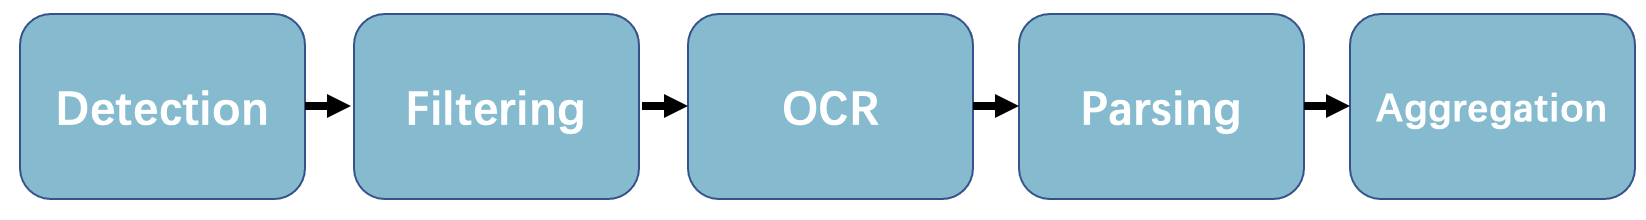
\includegraphics[width=0.8\columnwidth]{archi.png}  
   
	\caption{Architecture of pipeline}
\end{figure}

\section{Data analysis}

The original data we have consist of 1000 images for our Scene Text Recognition task, which was provided by our cooperate company -GLORY.ltd. In each image, there exists one or several carton boxes in a warehouse. Types of text information were printed on the carton boxes such as QR Code, Japanese characters, cargo volume and our target text: Date.
All the images has been manually labeled with several bounding boxes and text information annotations:date or non-date shown as Fig.3.

Based on the bounding boxes and annotations, we built a dataset used for the following several sections. This dataset contains over thousands of boxes, each box corresponds to an annotation. If the annotation is date, there would also exist a valid date text as the label.

\begin{figure}[ht] \centering
	\label{dataset}
	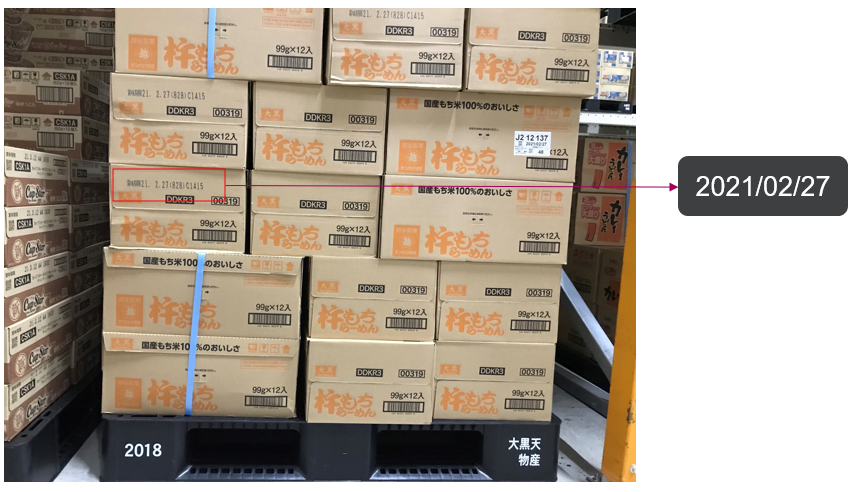
\includegraphics[width=0.8\columnwidth]{dataset.png}
	\caption{original image sample and a bounding box with corresponding label of date}
\end{figure}

\begin{figure}[ht] \centering
	\label{filtering}
	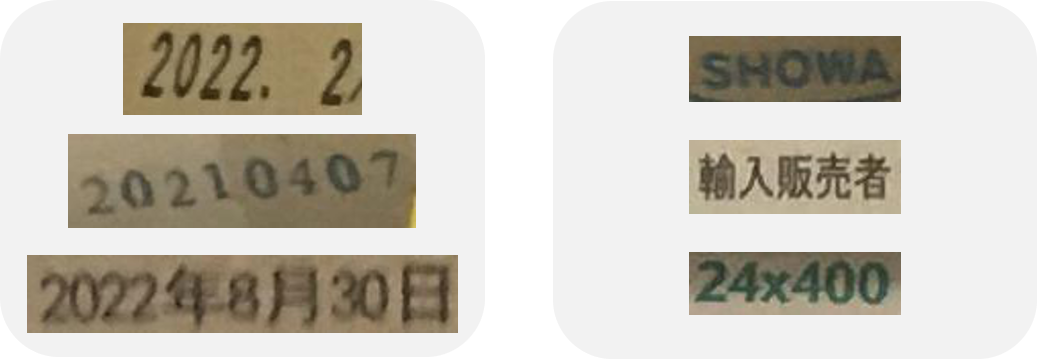
\includegraphics[width=0.8\columnwidth]{filter.png}
	\caption{date boxes (left) and non-date boxes (right) in filtering dataset}
\end{figure}

The difficulty for recognizing the date on the original image mainly existed in two parts:First is how to correctly filter the useless information like QR Code, second is recognizing the digital of date and translate it. To solve those problem, we developed the following pipeline.

\section{Proposed Pipeline/Methodology}

In this part, we will introduce our entire pipeline.

\subsection{Text Detection}

In the first step, we used the Easy-OCR, a library in python, to finish the detection of text in image. The output image after detection is illustrated++ as Fig.3. All the text has been marked with green boxes. Then the second step, all the marked text will be cropped from original image and saved in the disk. The cropped boxes will be used in the second step: Filtering.

\begin{figure}[ht] \centering    
	\label{detection}     
	\includegraphics[width=0.8\columnwidth]{detection.png}  
   
	\caption{image after detection marked with green bounding boxes}
\end{figure}

\subsection{Date Text Filtering}

In the filtering part, we trained a binary classification model as ResNet-50 on the data-set provided by our cooperate company. this sub-set include 2 types of boxes, one is our target date boxes, and the other is no-date boxes which need to be removed from all the boxes. In fig.4, we present several boxes in filtering data-set which left is date and right is non-date.

\begin{figure}[ht] \centering    
	\label{filtering}     
	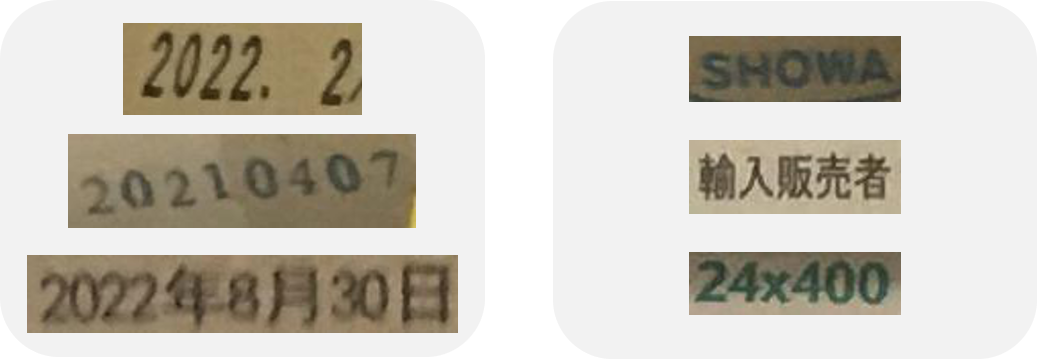
\includegraphics[width=0.8\columnwidth]{filter.png}  
   
	\caption{date boxes (left) and non-date boxes (right) in filtering dataset}
\end{figure}

The classifier has been well trained so that we could filter the useless texts from our crops get from the second step.

\subsection{Date Recognition}

Once we finished filtering the boxes and get only the date images, We will use an deep learning model which name is STAR-Net and its pre-trained weight to recognize all the date images. To make the recognition process effective and accurate enough, a series of experiments has been set to modify the model here, we will introduce the details of experiment in the next section.\par
In this part, the date boxes would be translated into text consist of digital and punctuation illustrated as Fig.5

\begin{figure}[ht] \centering    
	\label{recognition}     
	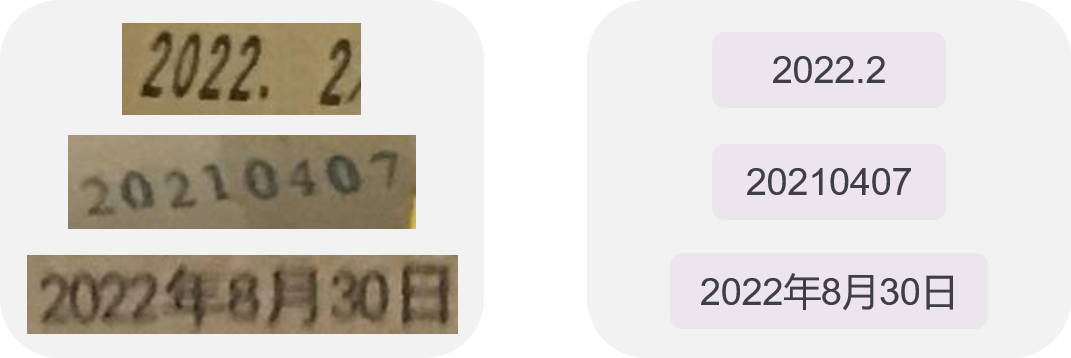
\includegraphics[width=0.8\columnwidth]{recognition.png}  
   
	\caption{date boxes (left) and recognition model outputs(right)}
\end{figure}

\subsection{Regular Expression Parsing(more explanation)}

In this part we generate the regular expression to parse our model outputs to dates, all the output of model will be transformed into an uniform format : Year Year Year Year/Month Month/Day Day.

Regular Expression is  used to standardize a canonical expression, and it has properties and methods to check whether the given string conforms to the rules.\par

\begin{figure}[ht] \centering    
	\label{parsing}     
	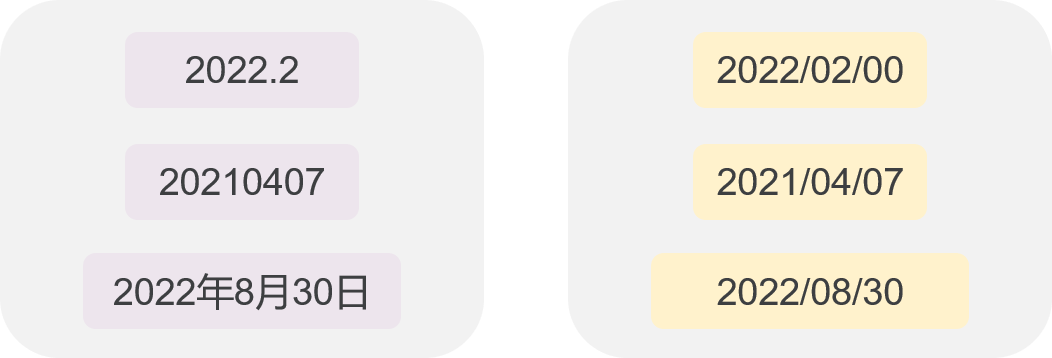
\includegraphics[width=0.8\columnwidth]{parsing.png}  
   
	\caption{recognition model outputs(right) and date after regular expression parsing}
\end{figure}

\subsection{Result Aggregation(more explanation)}

In our dataset, there are some images appear several times corresponding to a same ground-truth dates and index, so we need to select a highest repetition result as the only output for those images

\begin{figure}[ht] \centering    
	\label{aggregation}     
	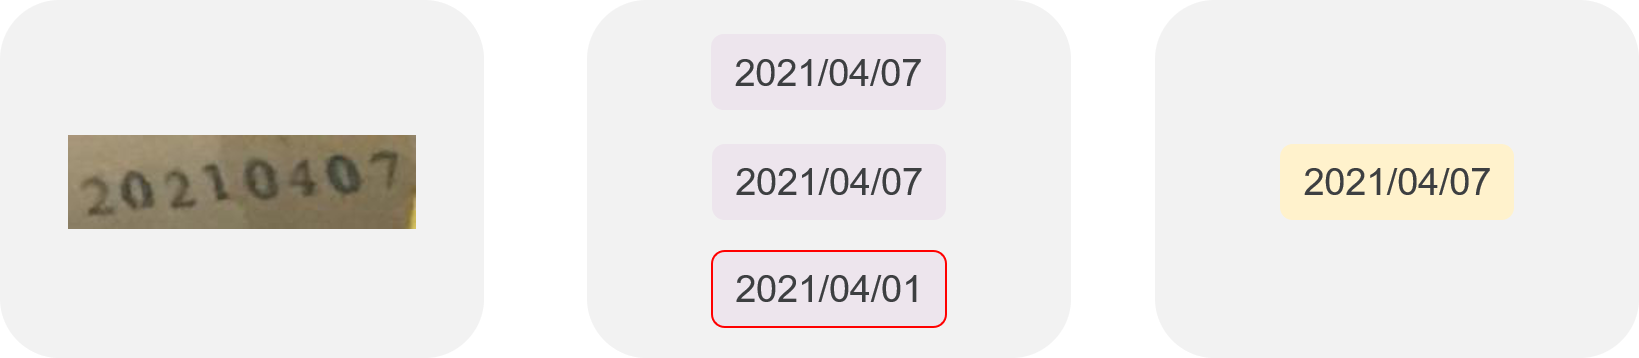
\includegraphics[width=0.8\columnwidth]{aggre.png}  
   
	\caption{aggregate several repeat outputs to one}
\end{figure}

\section{Experiments}

To built a high accuracy Scene Text Recognition system, we set a series of experiments to modify each part inside our pipeline. 

\subsection{Experiment Environment}

We simply use 4 GTX 1080Ti GPUs with 12 GBs for pre-training and fine-tuning for all the experiments. 
The Table.1 present the experiment parameter details in our paper.

\begin{table}[]
\centering
\begin{tabular}{l|l|l}
               & Filtering & Recognition \\ \hline
Baseline Model & ResNet-50 & STAR-Net    \\ \hline
Batch Size     & 256       & 192         \\ \hline
Optimizer      & SGD       & Adadelta    \\ \hline
Loss Function  & CE Loss   & CE Loss     \\ \hline
Learning Rate  & 0.01      & 1           \\ \hline
Training Epoch & 60        & 150         \\ 
\end{tabular}
\caption{Experiment settings}
\label{Experiment settings}
\end{table}

\subsection{Filtering model Training}

In this part, we trained a binary classifier specifically to do this filtering task. Here we choose ResNet-50 as the main architecture. For this dataset, we randomly choose $85\%$ as the training set and $15\%$ as the validation set, then training the model on the training set from the initial weight. After 60 epochs, the test accuracy has archived $99.8\%$ shown as fig.8. This result is good enough to remove almost all the non-date boxes.

\begin{figure}[ht] \centering    
	\label{filtering model}     
	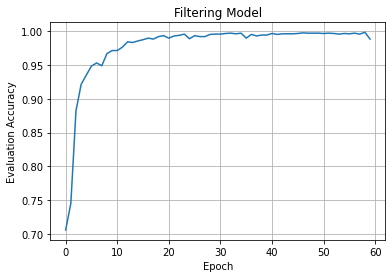
\includegraphics[width=0.8\columnwidth]{filtering model.png}  
	\caption{validation accuracy of filtering model}
\end{figure}

\subsection{Date Recognition Experiments}

In the date recognition part, we set up two sets experiments to achieve the highest recognition accuracy.

\subsubsection{Baseline model comparison}

To start the process of date recognition, we selected several existing OCR models. We verified the performance of these models on our dataset based on pre-trained models and without fine-tuning, then finally selected the best one as our baseline model.The Fig.9 present the validation accuracy of different model.

\begin{figure}[ht] \centering
	\label{baseline model}     
	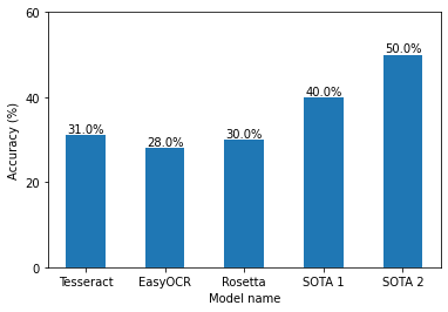
\includegraphics[width=0.8\columnwidth]{baseline model.png}  
	\caption{validation accuracy of baseline OCR model without fine-tuning}
\end{figure}

In this figure, pytesseract is a traditional OCR model developed by HP Labs and now maintained by Google, while EasyOCR and Rosseta are two general wild OCR models. Meanwhile, the second most effective model is STAR-Net, developed by Wei Liu et al. in 2016. the final best model was optimized in 2019 by Jeonghun Beak et al. by replacing the Connectionist Temporal Classification (CTC) in the STAR-Net model. Classification (CTC) was replaced with Attention-based Sequence Prediction (Attn).

Both models achieved the best results in the paper:"What Is Wrong With Scene Text Recognition Model Comparisons?Dataset and Model Analysis", based on the generic datasets: MJSynth [Max et al., 2014] , SynthText [Ankush et al.2016]. So to distinguish these two models, we will refer to them as State-Of-The-Art 1 and State-Of-The-Art 2, respectively.

Based on this result, our next experiments will use STAR-Net as a baseline

\subsubsection{Separator Strategy}

In our dataset, many dates correspond to labels that contain many punctuation marks or Japanese kanji in addition to numbers. Therefore, when starting the recognition task, we assume two cases to recognize date images: the first one is to ignore all punctuation marks and replace all labels in the training set with a special separator Sep to match the punctuation and kanji, and then fine-tune our model based on the new labels, which we call the first strategy One-Sep strategy. the second one is to recognize all We call the first strategy One-Sep strategy. The second one recognizes all punctuation marks, keeping the original labels for each one, and fine-tunes the model based on them, which we call All-Sep strategy.

Based on the 2 strategies and 2 models SOTA1 and SOTA2, we did 4 experiments with the same parameters, and the f Table.2 shows the results of the experiments. 

\begin{table}[]
\centering
\begin{tabular}{l|l|l|l}
        & SOTA1 & SOTA2 &   \\ \hline
One-Sep & 0.858 & 0.863 &   \\ \hline
All-Sep & 0.866 & 0.880 &   \\ 
\end{tabular}
\caption{Separator Experiment Results}
\label{Separator Experiments}
\end{table}

\subsection{Error Analysis}

In the previous sub-section, we obtained the highest recognition rate as $88\%$. In addition to the experiments mentioned in this paper, we also fine-tuned some of the parameters in the experiments, but it did not lead to a significant improvement in the recognition rate. Therefore, we performed an error analysis for the SOTA2+All-sep experiments and summarized the wrong predictions into several aspects, as Fig.10-Fig13 shown.

\begin{figure}[ht] \centering    
	\label{pattern errors}     
	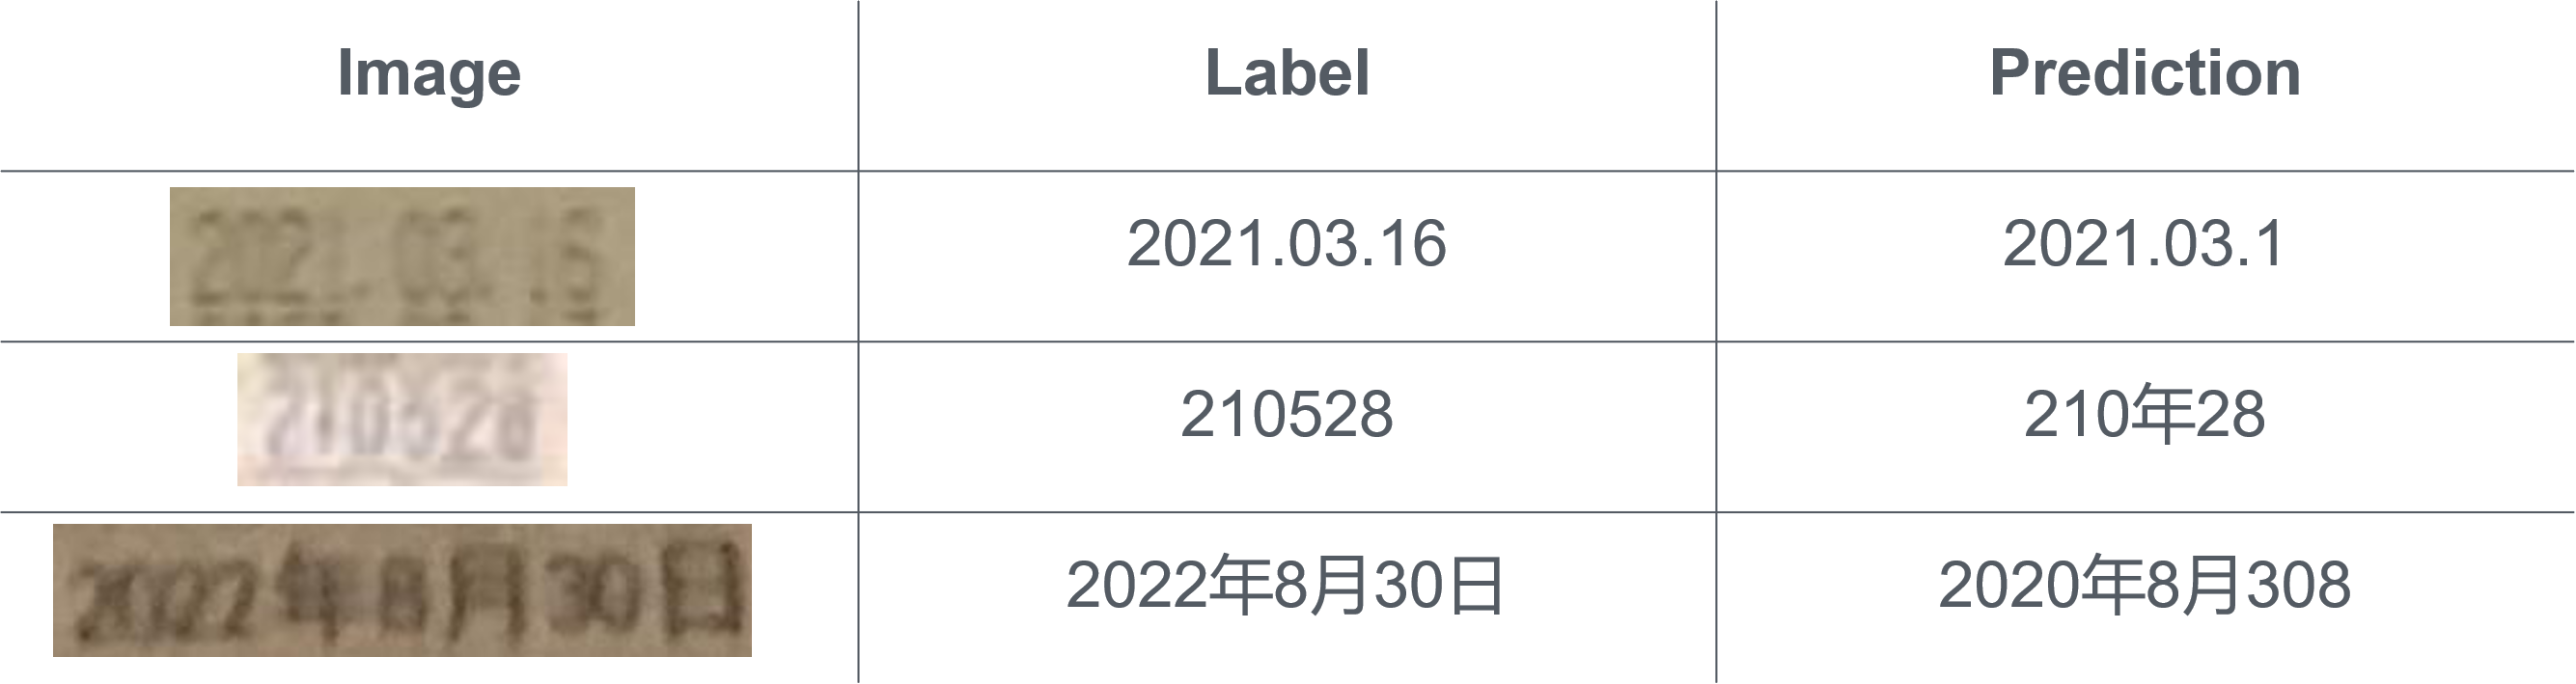
\includegraphics[width=0.8\columnwidth]{pattern.png}
	\caption{Pattern Errors}
\end{figure}

\begin{figure}[ht] \centering    
	\label{number errors}     
	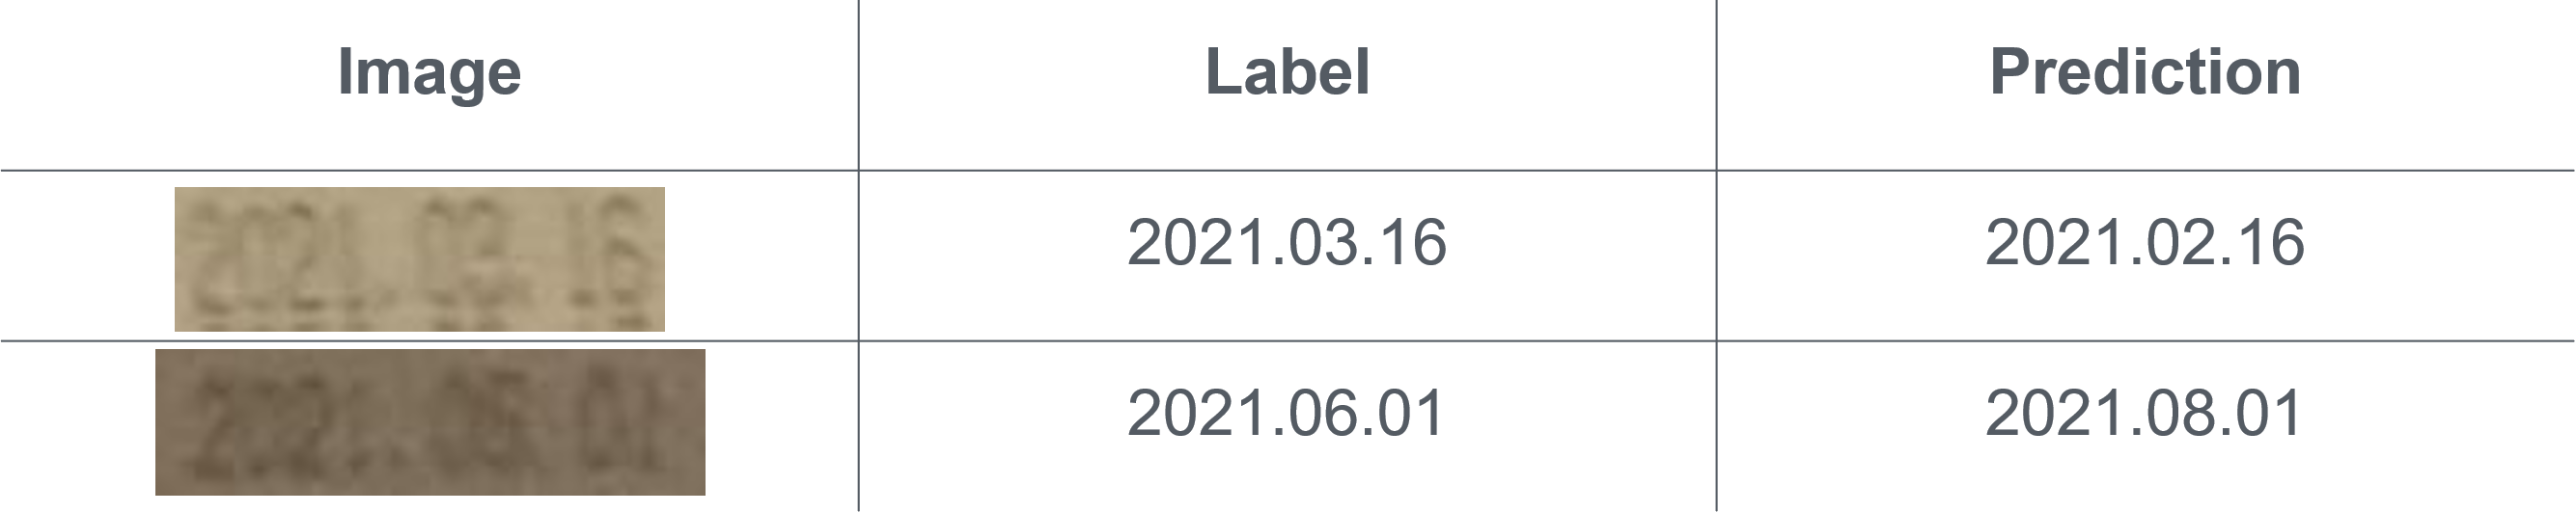
\includegraphics[width=0.8\columnwidth]{number.png}
	\caption{Number Errors}
\end{figure}

\begin{figure}[ht] \centering    
	\label{separator errors}     
	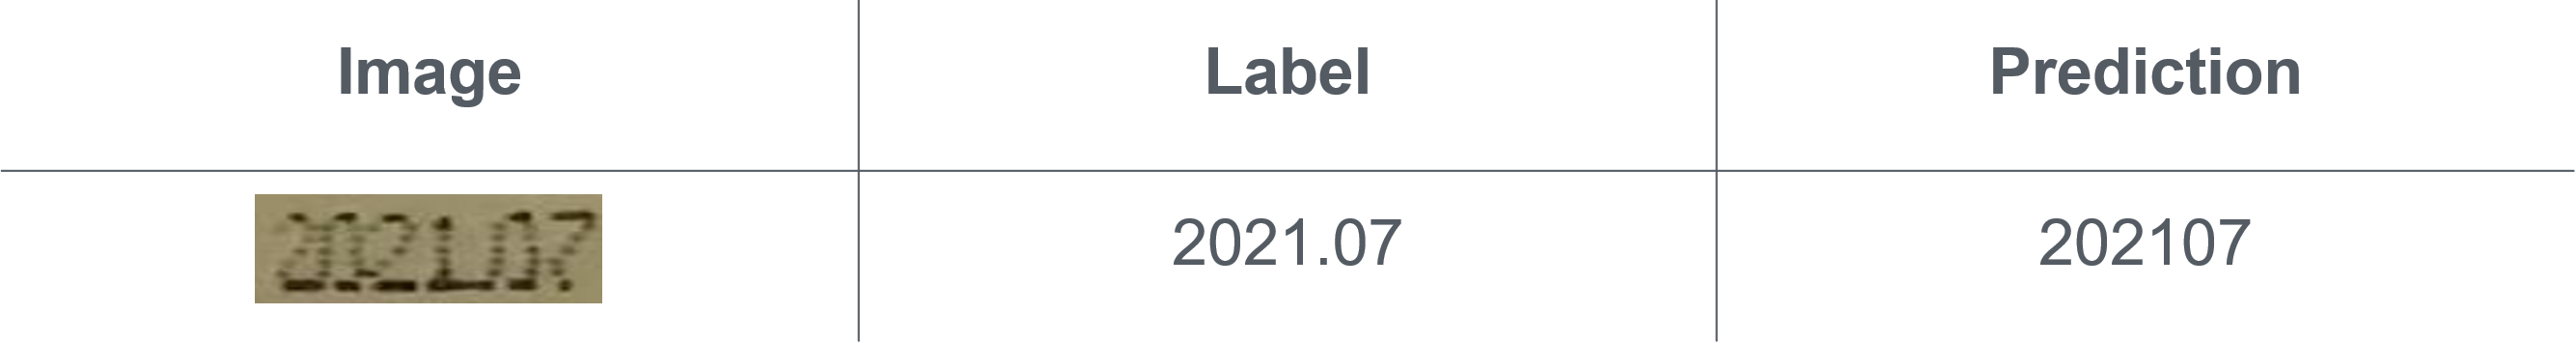
\includegraphics[width=0.8\columnwidth]{separator.png}
	\caption{Separator Errors}
\end{figure}

\begin{figure}[ht] \centering    
	\label{special sample}     
	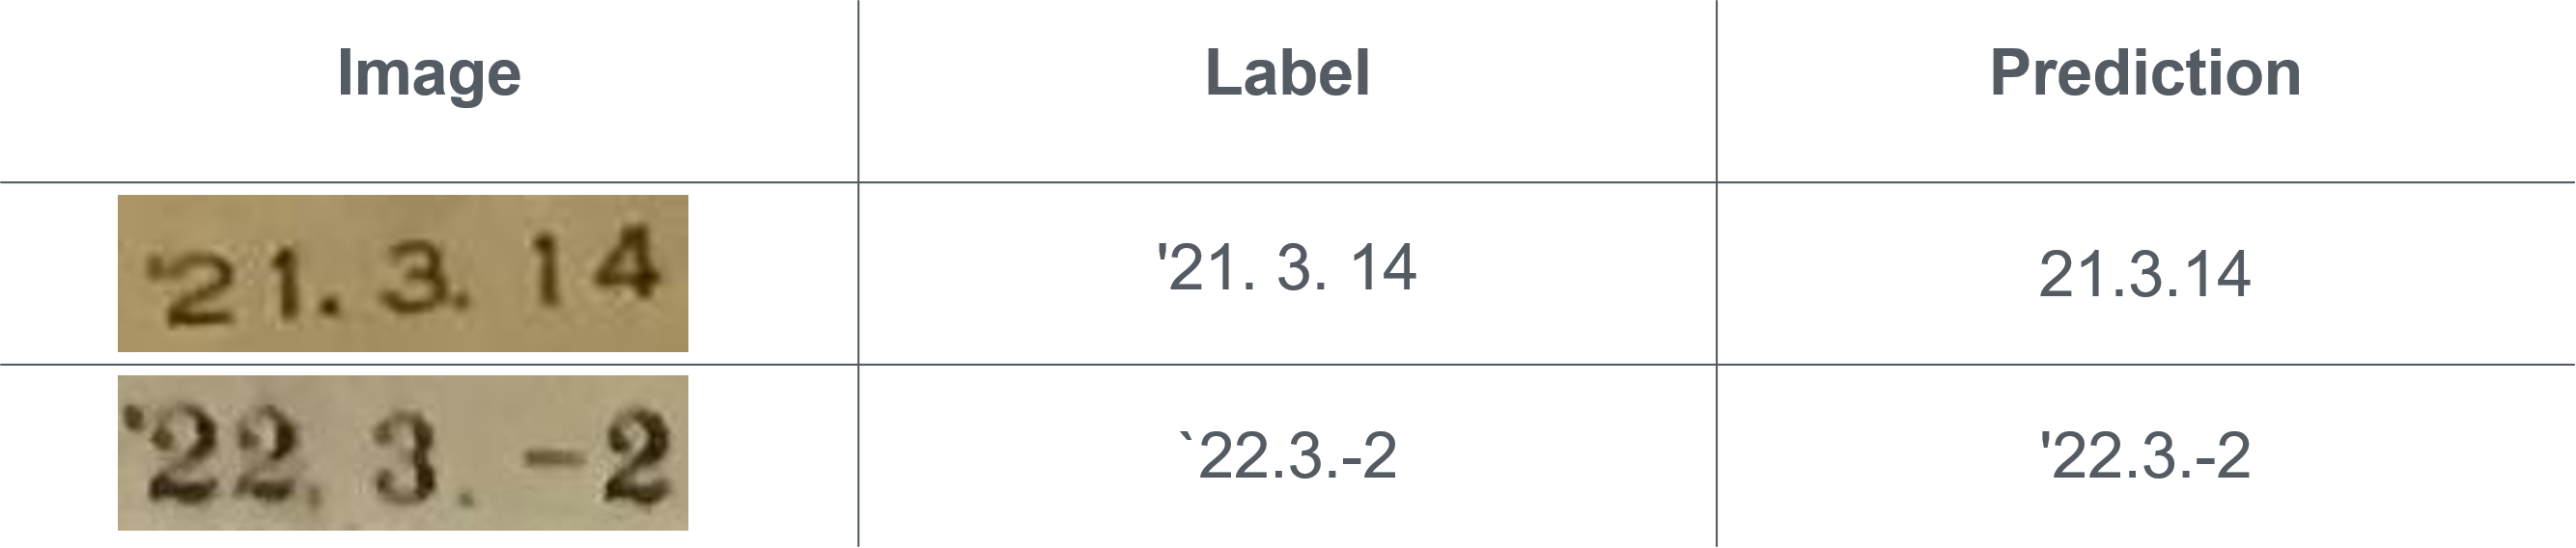
\includegraphics[width=0.8\columnwidth]{special sample.png}
	\caption{Special Sample}
\end{figure}

For the above four types of errors, the first pattern error and the second number error mainly originate from the recognition process, the image is too blurred and not easy to fix, the third separator error is also caused by the image quality, but can be completely fixed by Regular Expression Parsing, and the fourth special The fourth special case is difficult to fix, but the number of this case is small enough to be ignored.

So in the next sub-section, we will focus our attention on the first and second types of errors

\subsection{Proposed Method}

The type 1 and 2 errors usually do not correspond to the valid date shown as Fig.10. These types of errors are difficult to be parsed by Regular Expression due to the missing numbers or misplaced separators.
Therefore, we hope to apply the function of parsing to the recognition process of the model by using parsing to filter out those predictions that do not conform to the Regular Expression then output the highest probability sequence that matches the Regular Expression.\par

In our recognition model, the sequence model gives a probability matrix before outputting the final prediction, which corresponds to the sequence length of the predicted text and the probability of each time-step on the sequence corresponding to all elements in the dictionary. In the original STAR-Net model, the authors directly used the Greedy decoding strategy which means each time-step on the sequence is directly selected as the character of the time-step with the highest probability. However, for our method, the text sequence with the highest probability selected by this decoding strategy does not match the Regular Expression, and we want to use the parsing process to filter all possible text sequences. Therefore, we use the idea of beam search in the process of decoding. After getting all the sequences corresponding to the prediction results, we convert them directly into text format as the combination of digital and separator, and parse them by Regular Expression. The texts that can be parsed are retained, while the others are removed, and finally, for all the texts that pass parsing, we select the most probable one as the final output of the model.

In this way, we improved the accuracy of the recognition model from $88.8\%$ to $91\%$. The fixed prediction is shown in the Table.3 below.

\begin{table}[]
\centering
\begin{tabular}{c|c|c|c}
  & Errors     & Label      & Fixed Errors \\ \hline
1 & 210.02     & 21.02.02   & 2021/02/02   \\ \hline
2 & 2021.03.77 & 2021.03.07 & 2021/03/07   \\ \hline
3 & 2021133    & 202113     & 2021/01/03        
\end{tabular}
\caption{errors fixed by our methods}
\label{fixed errors}
\end{table}
\section{Related work(unfinished)}

details of traditional OCR system \par
introduction of What Is Wrong With Scene Text Recognition Model Comparisons

The paper What is wrong with xxxx provide us an effective framework to evaluate most of the existing STR model.

Transformation is a module to translate all the original images into normalized images. The text in the actual scene images usually appears in various shapes  such as curved and slanted, the different shapes of texts will cause the following part more difficult to extract the feature from the original image. So the thin-plate spline (TPS) transformation, a variant of the spatial transformation network (STN), has been implemented in the first part of the OCR model. the image after TPS process would be shown as Fig.5 

Fig.5 a curved image as the input of TPS, and a normalized image as the output. 

In the Feature Extraction stage, a CNN like ResNet would be used to extract the feature map from the normalized image getting from TPS. These features are used to estimate the character on each receptive field.

Then in the Sequence model stage, The STAR-Net used BiLSTM to reshape the extracted features from the second stage to be a sequence of features, each column in a feature map is used as a frame of the sequence. The Bidirectional structure could solve the problem like the lack of contextual information.

The last stage: Prediction. The STAR-Net provided 2 options for choosing, Contortionist temporal classification (CTC) and attention-based sequence prediction (Attn). However, the pre-trained weight they provided, only the Attn could recognize the punctuation like ',' or '.'. Due to the data we have was in the type of date, which include many punctuation and Japanese characters, we choose the Attn as the set of Prediction Stage.

\section{Conclusion and Future work}

In this paper, we present our pipeline, an combination of several deep learning models for recognizing the structure text in the actual scenes. Currently existed STR model did not provide a effective method to recognize the structure text, so we set ourselves a goal to develop a pipeline that could help users to extract the target structure text information from images with complicated environment and translated the text into uniform format. Our pipeline consist of 5 parts to do the STR task: Detection and filtering help users to extract the target texts boxes from original image, Date Recognition translate the target boxes into computer text format, finally the Parsing and Aggregation would transform kinds of different texts into uniform format and choose the correct one as the final output. Experiments results show that our pipeline has archived a pretty good accuracy based on our dataset. We believe that this pipeline could help both the users and researchers in the Scene Text Recognition (STR) field.

For future research, we will constantly modify our pipeline to improve the accuracy, such as replace the backbone OCR model by Tr-OCR, a current State-of-the-art Transformer-based OCR model for text recognition.

For lack of a common dataset of structure text, we also welcome other researchers in this field to use and comment on our pipeline, and we will continue to improve our pipeline to address those issues.


% References should be produced using the bibtex program from suitable
% BiBTeX files (here: strings, refs, manuals). The IEEEbib.bst bibliography
% style file from IEEE produces unsorted bibliography list.
% -------------------------------------------------------------------------
\bibliographystyle{IEEEbib}
\bibliography{icme2020template}

\end{document}
